\documentclass[11pt]{article}

\usepackage[review]{acl}

\usepackage{times}
\usepackage{latexsym}

\usepackage[T1]{fontenc}

\usepackage[utf8]{inputenc}

\usepackage{microtype}

\usepackage{inconsolata}

\usepackage{graphicx}

\usepackage{booktabs}          % \toprule / \midrule / \bottomrule din tabele
\graphicspath{{figures/}}      % beeswarm.png, fig_corr_matrix.png, fig_confusion.png

\title{Cross-Lingual Transfer for Romanian Lexical Complexity Prediction:
Fusing a Multilingual Encoder, a Language Model, Surprisal, and Eye-Tracking}

\author{}

\begin{document}
\maketitle
\begin{abstract}
Lexical complexity prediction is normally solved by fine-tuning an
encoder on annotated data in the target language, which excludes every
language that has none. We predict the lexical complexity of Romanian
words in context without using a single Romanian training label, by
fusing four signals that carry complexity knowledge from outside the
language: cross-lingual transfer through a frozen multilingual encoder
trained on English and Romance annotations, a complexity rating and
token surprisal from a Romanian language model, and a reading-effort
score derived from eye-tracking. The system reaches $69.74$ on the
shared-task metric, against $10.27$ for surface features alone, and
Pearson $r = 0.913$ on held-out Romanian items. The largest single gain
($+4.09$) comes from a lemma-frequency correction that repairs the
frequency estimates inflection corrupts, and transfers to any
morphologically rich language served by the same frequency lists. We
also report two negative results: with no target labels, fine-tuning
the encoder is consistently worse than freezing it, and in-source
validation does not predict transfer quality.
\end{abstract}

\section{Introduction}
\label{section:intro}

Text is only as accessible as its hardest words. Automatic simplification
replaces or explains the words a reader will struggle with, readability
assessment estimates whether a document suits its audience at all, and
material for language learners has to be graded to the learner's level;
all three rest on first deciding which words are hard, and for whom,
which is why complexity prediction is typically the first stage of a
simplification pipeline \citep{qiu-etal-2024-complex}. Lexical complexity
prediction (LCP) is the task that supplies this judgement: given a target
word in context, predict a continuous complexity score.

The field has converged on a single recipe for producing that judgement.
A decade of shared tasks --- from complex word identification
\citep{yimam-etal-2018-report} to the continuous formulation of CompLex
and SemEval-2021 \citep{shardlow-etal-2021-semeval} --- established that
the way to build an LCP system is to fine-tune a pretrained encoder on
complexity annotations in the language one cares about. The recipe works,
and it is expensive: each new language requires its own annotation
effort, as the recent Catalan, Spanish, Mandarin and Cantonese resources
illustrate \citep{saggion-etal-2024-lexical, qiu-etal-2024-complex}. It
also silently assumes the one resource most languages do not have.
Surveying the LCP datasets published between 2018 and 2024,
\citet{shardlow-etal-2024-multilingual} find nine of them, covering eight
languages. A language outside that set has nothing to fine-tune on.

Romanian is such a language, and it makes the problem sharper than a
simple absence of data. Fourteen labelled Romanian target words exist,
enough to sanity-check a system but neither to train one nor to validate
one, so there is no development set on which any design decision can be
made. Romanian also breaks the single most reliable predictor of
processing difficulty. Word frequency governs how long readers fixate a
word \citep{rayner1998eye} and it is the top-ranked feature in our own
attribution analysis (Section~\ref{sec:results}), but Romanian is heavily
inflected and inflected forms are systematically missing from frequency
lists: of the 1587 Romanian target tokens in our test set, $11.7\%$ are
absent from the frequency list entirely and would be scored as maximally
rare, while for $36.0\%$ the lemma carries a higher frequency than the
inflected form --- by $0.86$ Zipf units on average. Ordinary words are
therefore made to look rare, and the words this happens to are precisely
the morphologically marked ones. A method for Romanian has to transfer
complexity knowledge from outside the language \emph{and} repair the
frequency signal it transfers on.

In this paper, we predict the lexical complexity of Romanian words in
context without a single Romanian training label, by fusing four
independent signals that each carry complexity knowledge from outside the
language. Our main contributions are:

\begin{itemize}
\item \textbf{A zero-label LCP system for Romanian.} It combines
  cross-lingual transfer through a frozen multilingual encoder, a
  language-model complexity rating, surprisal, and a reading-effort score
  derived from eye-tracking, and reaches $69.74$ on the shared-task
  metric --- against $41.76$ for a system restricted to the signals the
  shared task itself provides and $10.27$ for surface features alone ---
  and Pearson $r = 0.913$ on the 14 held-out Romanian items. To our
  knowledge, no prior system predicts lexical complexity for Romanian.

\item \textbf{A lemma-frequency correction for morphologically rich
  languages.} Substituting the lemma frequency when the inflected form is
  missing or rarer is worth $+4.09$, the largest single gain in the
  system, and applies to any inflected language served by the same
  frequency lists.

\item \textbf{An account of why the four signals compose rather than
  duplicate each other.} SHAP attributions and the inter-signal
  correlation matrix show that the cross-lingual signal is essentially a
  frequency detector, that the language-model rating and surprisal are
  near-independent ($r = 0.07$), and that eye-tracking contributes
  through its \emph{late} measures --- re-reading and incoming
  regressions --- the contextual-integration difficulty that none of the
  lexical signals capture.

\item \textbf{Two negative results with practical consequences.}
  Fine-tuning the encoder, full or LoRA, is consistently \emph{worse}
  than leaving it frozen ($0.461$ and $0.462$ against $0.515$ in-source),
  because without target labels it overfits the source language and
  degrades the multilingual alignment the transfer depends on. And
  in-source validation is an unreliable guide: three configurations that
  win on English-to-Romance transfer lose on Romanian.
\end{itemize}

Because Romanian offers no development set, three fusion weights were
selected against the public leaderboard score; we report every tuned
quantity, show that Pearson $r$ is invariant to the calibration step and
can therefore serve as the primary measure, and measure what the tuning
buys on labels it never saw --- $0.019$ of Pearson $r$
(Sections~\ref{sec:tuning} and~\ref{sec:14items}).

Our setting differs from the LCP literature in the resource it assumes
rather than in the model it uses. Work in the CompLex and CWI line trains
on target-language annotations, and the multilingual simplification
pipeline that extends this to ten languages
\citep{shardlow-etal-2024-bea} does not include Romanian; we instead
treat complexity as knowledge to be imported. Our use of gaze runs
opposite to the psycholinguistic literature, which predicts reading times
from model surprisal \citep{hollenstein-etal-2021-multilingual}: we
invert the direction and read gaze as evidence about complexity. And
where cross-lingual transfer is normally realised by fine-tuning on the
source language \citep{pires-etal-2019-multilingual}, we find the frozen
encoder to be the stronger choice in the zero-label regime.
Section~\ref{sec:related} sets these differences against the specific
work they concern.

Section~\ref{section:approach} describes the four signals, how they are
combined, and exactly what was tuned; Section~\ref{sec:results} reports
the ablation, the evaluation on the 14 Romanian items and the
interpretability analysis; Section~\ref{sec:negative} collects what did
not work; Section~\ref{section:conclusions} concludes; and the
Limitations section states what the setting cannot support.

% =====================================================================

\section{Related Work}
\label{sec:related}

\paragraph{Lexical complexity prediction.}
CWI was originally posed as classification over annotated target words
\citep{yimam-etal-2018-report}; SemEval-2021 Task~1 replaced it with a
continuous scale on the CompLex corpus
\citep{shardlow-etal-2021-semeval}, which is the formulation we adopt.
Zero-shot evaluation is not itself new to the task: the 2018 shared task
already included a multilingual track whose French test set came with no
French training data. That setting is a considerably easier one than
ours, however --- it asked for binary and probabilistic classification
rather than continuous prediction, and it supplied annotated training
data in three languages, one of them Romance. Coverage has since grown to
Catalan, Spanish, Mandarin and Cantonese
\citep{saggion-etal-2024-lexical, qiu-etal-2024-complex} and to the ten
languages of the MLSP shared task \citep{shardlow-etal-2024-bea}, but the
review of \citet{shardlow-etal-2024-multilingual} shows annotated LCP
data still concentrated in a few high-resource languages. Romanian
appears in none of these resources, and we are aware of no published LCP
system for it. We use the English and Romance portions of these resources
as the source side of our transfer.

\paragraph{Cross-lingual transfer without target labels.}
Multilingual encoders such as XLM-R \citep{conneau2020xlmr} place
translation-equivalent words close together, which makes zero-shot
transfer of a regressor trained on one language plausible. Transfer
quality is far from uniform across languages, however, and degrades for
languages with less pretraining data and richer morphology
\citep{pires-etal-2019-multilingual, wu-dredze-2020-languages} ---
precisely the regime Romanian occupies. Transfer is moreover normally
realised by fine-tuning the encoder on the source language; that feature
extraction can outperform fine-tuning when the target task is distant
from the source is known \citep{peters-etal-2019-tune}, but we are aware
of no prior report of it for cross-lingual complexity transfer, where we
measure the gap at $0.515$ against $0.461$ in-source. This motivates both
our frozen-encoder design and the lemma-frequency correction: the encoder
supplies cross-lingual semantics, and the correction repairs the lexical
feature that morphology corrupts.

\paragraph{Surprisal and eye movements as difficulty signals.}
Surprisal theory predicts that processing effort scales with the
negative log probability of a word in context \citep{hale2001probabilistic},
and gaze measures --- longer fixations, re-reading, regressions ---
are the standard behavioural correlate of that effort
\citep{rayner1998eye}. Language-model surprisal predicts reading times
across languages \citep{hollenstein-etal-2021-multilingual}, including
in Romance languages \citep{alves-2025-benchmarking}. Both literatures
run from text to behaviour; we take the converse view. Because surprisal
and gaze both track processing difficulty, and because neither requires
complexity annotation, both can serve as label-free signals for
complexity in a language that has no annotated data.

\paragraph{Evaluation without a development set.}
Selecting a model against the same data used to report its score
inflates that score, and the effect is well documented for standard
splits and shared-task leaderboards \citep{gorman-bedrick-2019-need}.
A zero-label setting has no honest alternative to offer --- there is no
development set to tune on --- so we follow the recommendation to state
the selection procedure explicitly and to quantify its effect
(Section~\ref{sec:tuning}).

\paragraph{Romanian resources.}
The Romanian signals in our system come from RoLlama3
\citep{masala-etal-2024-vorbesti}, an open-weights Romanian
instruction-tuned model, which we query both for an explicit
complexity rating and for raw token surprisal. All model outputs are
interpreted with SHAP \citep{lundberg2017shap}.

\section{Approach}
\label{section:approach}

\subsection{Task, data and metric}

Given a target word in a Romanian sentence, the task is to predict a
complexity score in $[0,1]$, where $0$ is a fully familiar word and $1$
a maximally difficult one. The test set contains $1587$ target words.
Fourteen Romanian items carry gold complexity labels; they are too few
to train or validate on, and we use them only as an independent check
(Section~\ref{sec:14items}). Aggregated eye-tracking measurements over
the same texts are distributed with the task, so gaze is available for
the target words without any annotation effort of our own.

Systems are ranked by
\begin{equation}
  \label{eq:metric}
  \mathrm{score} = 50\,\bigl(|r| + \max(0, R^2)\bigr),
\end{equation}
where $r$ is the Pearson correlation with the gold scores and $R^2$ the
coefficient of determination. This is the metric defined by the shared
task, not a standard LCP measure, and it conflates two different
things: $|r|$ rewards ranking the words correctly, while $R^2$ rewards
putting them on the right absolute scale. We report it because the
leaderboard returns only this composite --- the gold labels for the
test set are not released, so we cannot decompose our own submissions
into $r$ and $R^2$. Wherever labels are available we report $r$
separately, and we take $r$ as the primary measure for the reason given
in Section~\ref{sec:tuning}.

\subsection{Setup and in-source validation}

The system uses XLM-RoBERTa-base \citep{conneau2020xlmr} and RoLlama3-8B
\citep{masala-etal-2024-vorbesti} in 4-bit quantisation, with
\texttt{transformers}, \texttt{scikit-learn} and \texttt{wordfreq}.

With no Romanian labels to validate on, design decisions were made
\emph{in-source}: a regressor is trained on one set of source languages
and evaluated on another, with cross-validation inside each source. We
report two such quantities, and they are not interchangeable.
$r_{\mathrm{EN}\rightarrow\mathrm{RO}^{*}}$ is the correlation obtained
when training on English CompLex \citep{shardlow-etal-2021-semeval} and
testing on the Romance portion of MLSP \citep{shardlow-etal-2024-bea};
$\bar{r}_{\mathrm{transfer}}$ averages that with the reverse direction.
Built on thousands of real labels, either check tells us whether a
configuration is sound before it is applied to Romanian. Its limits are
the subject of Section~\ref{sec:negative}.

\subsection{The four signals}

Each signal estimates complexity in a different way, and none of them
requires a Romanian complexity annotation.

\paragraph{(A) Cross-lingual transfer.}
Complexity is learned from English and Romance annotations
\citep{shardlow-etal-2021-semeval, shardlow-etal-2024-bea} and carried
over to Romanian through the shared representation space of
XLM-RoBERTa, which places translation-equivalent words close together
(Section~\ref{sec:related}). A Ridge and HistGradientBoosting blend
reads each word's embedding --- the mean of the last four layers,
centred per language --- together with a few surface cues: frequency,
length, syllable count and capitalisation.

One Romanian-specific correction accounts for the largest single gain
in the system. Because Romanian is heavily inflected, many word forms
are absent from the frequency list and would be scored as maximally
rare: of the $1587$ target tokens, $11.7\%$ have no entry at all, and
for $36.0\%$ the lemma is more frequent than the inflected form, by
$0.86$ Zipf units on average. We therefore use
$\max\bigl(\mathrm{zipf}(\mathrm{form}), \mathrm{zipf}(\mathrm{lemma})\bigr)$
in place of the form frequency. Section~\ref{sec:14items} identifies the
condition under which this substitution is the wrong thing to do.

\paragraph{(B) Language-model rating.}
RoLlama3 is asked to rate the target word in context on a $1$--$5$
scale. We read the answer from the probabilities the model assigns to
the five digit tokens rather than from the text it generates, which
turns a discrete choice into a smooth expected value.

\paragraph{(C) Surprisal.}
Surprisal, $-\log P(w \mid \mathrm{context})$, measures how unexpected
the word is; under surprisal theory an unexpected word is harder to
process \citep{hale2001probabilistic}. It comes from the same forward
pass as (B) but is a raw internal statistic, which is why it is nearly
independent of the rating ($r = 0.07$).

\paragraph{(D) Eye-tracking.}
Harder words are fixated longer and re-read more often
\citep{rayner1998eye}. We compress the eight per-word effort measures
into a single reading-effort score with PCA. The first component
explains $62\%$ of the variance and every measure loads on it with the
same sign (Table~\ref{tab:pca}), so the component is interpretable as a
single ``more effort $=$ more complex'' axis.

\subsection{Fusing the signals}

The four signals live on different scales, so each is standardised and
they are combined as a weighted average. Signal A is itself an ensemble
of the English-source and Romance-source transfers, averaged after
standardisation. The fused score is then mapped onto the scale of the
test distribution,
\begin{equation}
  \label{eq:calib}
  \hat{y} = \mathrm{clip}\bigl(\mu + \sigma \cdot z(s),\; 0,\; 1\bigr),
\end{equation}
with $\mu = 0.27$ and $\sigma = 0.125$. Per-signal weights are in
Table~\ref{tab:signals}.

\subsection{What was tuned, and what it costs}
\label{sec:tuning}

A zero-label setting has no development set, and selecting anything
against the evaluation score is a known way to inflate it
\citep{gorman-bedrick-2019-need}. We state exactly what this affects.

Five numbers in the system were chosen against the public leaderboard
score: the three fusion weights and the two constants of
Equation~\ref{eq:calib}. The weights were searched on a coarse grid;
for the eye-tracking weight the full sweep was
$w_D \in \{0, 0.10, 0.20, 0.30\} \rightarrow 68.90, 69.66, 69.74,
69.00$. Everything else --- the encoder, the layer, the feature set,
the regressor, the lemma correction --- was decided in-source, without
reference to the leaderboard.

Two things bound the damage. First, the calibration constants cannot
affect $r$ at all. Equation~\ref{eq:calib} is affine up to the clip,
and the clip is inactive on our predictions, whose range is
$[0.014, 0.845]$; Pearson $r$ is invariant under affine rescaling, so
$\mu$ and $\sigma$ --- the two quantities that most directly encode
information about the test distribution --- move only the $R^2$ term of
Equation~\ref{eq:metric}. This is why we treat $r$ as the primary
measure. Second, the response surface is flat: the eye-tracking sweep
spans $0.84$ points end to end, and on the 14 Romanian items the tuned
weights are worth $0.019$ of Pearson $r$ over uniform weights
(Section~\ref{sec:14items}). The one number that must be read as an
upper bound is the $+0.84$ attributed to eye-tracking in
Table~\ref{tab:ablation}: it is the maximum of the sweep that selected
$w_D$, and no independent estimate of it is available.

\section{Results}
\label{sec:results}

\subsection{How much each signal contributes}

Table~\ref{tab:ablation} builds the system one signal at a time.
Restricted to what the shared task itself provides --- surface features
and eye-tracking --- the system reaches $41.76$; the imported signals
take it to $69.74$, so roughly $40\%$ of the final score is
attributable to knowledge brought in from outside Romanian. Surface
features alone reach $10.27$. The single largest step is adding the
cross-lingual and language-model signals together ($+22.76$); the
lemma-frequency correction is the largest single gain after that
($+4.09$), and surprisal and eye-tracking each add a small amount.

\subsection{Evaluation on the 14 Romanian items}
\label{sec:14items}

The fourteen labelled Romanian items are the only real Romanian
supervision in existence for this task. They were never used for
training and took no part in weight selection, which was carried out
against the leaderboard; they were consulted during development as a
sanity check, so they are not a pristine test set either, but they are
independent of the tuning audited in Section~\ref{sec:tuning}.
Table~\ref{tab:ro14} reports Pearson $r$ on them. Two caveats apply
throughout: $n = 14$, so the confidence intervals are wide; and only
signals A and B are available on these items, because surprisal was
never computed for them and only $2$ of the $14$ carry eye-tracking.

The fused signal reaches $r = 0.913$, and a permutation test rejects
chance at $p < 0.0001$ despite the sample size. Uniform weights give
$0.894$: the tuning is worth $0.019$, which is the estimate quoted in
Section~\ref{sec:tuning}. With the calibration constants of
Equation~\ref{eq:calib} the composite metric on these items is $73.53$
($R^2 = 0.558$), close to the $69.74$ obtained on the full test set and
in the same direction, which is weak evidence that the leaderboard
figure is not inflated.

\paragraph{A scope condition for the lemma correction.}
The first two rows of Table~\ref{tab:ro14} are the frequency baselines,
and they invert. Raw form frequency correlates $-0.606$ with
complexity, the expected direction; after the lemma correction the
correlation is $+0.092$. The reversal comes from a single item:
\emph{putu}, a simple-perfect verb form, is the most complex word in the
set ($0.545$) and the correction raises its frequency estimate by
$2.76$ Zipf units, turning the hardest word into one of the easiest.
Excluding it, the two baselines are $-0.465$ and $-0.476$, so on the
remaining thirteen items the correction is neutral to mildly helpful.
The correction assumes that an inflected form inherits its difficulty
from its lemma. That assumption fails exactly when the inflection is
itself the source of difficulty --- archaic, literary or otherwise
marked forms --- and Romanian simple-perfect verbs are such a case. The
$+4.09$ measured over $1587$ items says the assumption usually holds;
this item says it is an assumption, not an identity.

\subsection{What drives the prediction}

A SHAP analysis over named features (Figure~\ref{fig:beeswarm}) places
frequency first, the language-model rating second and surprisal third;
the surface features barely matter. Table~\ref{tab:signals} gives the
same ordering at the signal level, and it agrees with the tuned
weights --- SHAP describes the fitted model, it does not choose the
weights. The signals are complementary rather than redundant
(Figure~\ref{fig:corr}): the rating and surprisal are nearly
independent, while the cross-lingual signal tracks frequency closely
enough to be read as a frequency detector with semantics attached.

\subsection{Eye-tracking contributes through its late measures}

Eye-tracking helps because it carries something the lexical signals do
not, and the division is the one predicted by the reading literature.
Partialling out frequency and length from each gaze measure over the
$1509$ test words that have gaze data, the early measures --- first
fixation duration, first-pass reading time, skip rate --- retain almost
no relation to the system's prediction ($\bar{r} = 0.010$) or to
surprisal ($\bar{r} = -0.027$): what they encode is lexical access,
which signal A already knows. The late measures --- re-reading time,
incoming regressions, refixation rate --- retain $\bar{r} = 0.243$ and
$\bar{r} = 0.177$ respectively. Late gaze is where the
contextual-integration difficulty lives, and that is the part of the
eye-tracking signal that is not already in the other three. As a
separate check on the transfer regressor itself, on held-out English
words it sorts complexity into easy, medium and hard bands with a
clearly diagonal confusion matrix (Figure~\ref{fig:confusion}).

\begin{figure}[tbp]
\centering
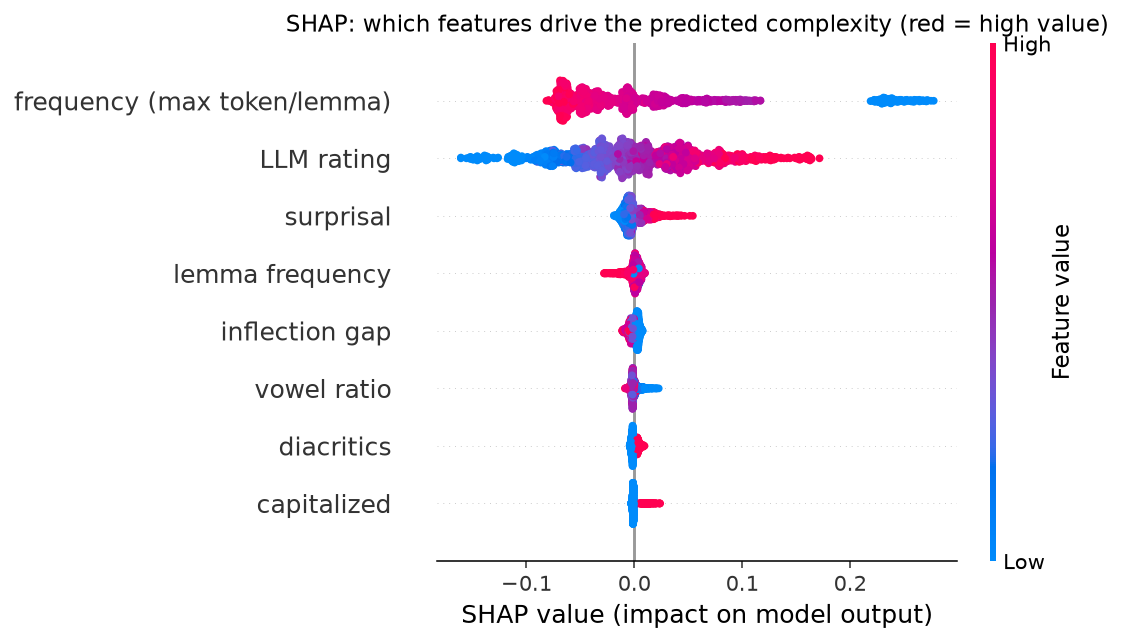
\includegraphics[width=\columnwidth]{beeswarm.png}
\caption{SHAP over named features (top 8 shown). Frequency dominates, then the LLM rating and surprisal. The
separate blue cluster on the frequency row is the group of very rare / out-of-vocabulary words, which push the
predicted complexity up --- the expected behavior. Red = high feature value.}
\label{fig:beeswarm}
\end{figure}

\begin{figure}[tbp]
\centering
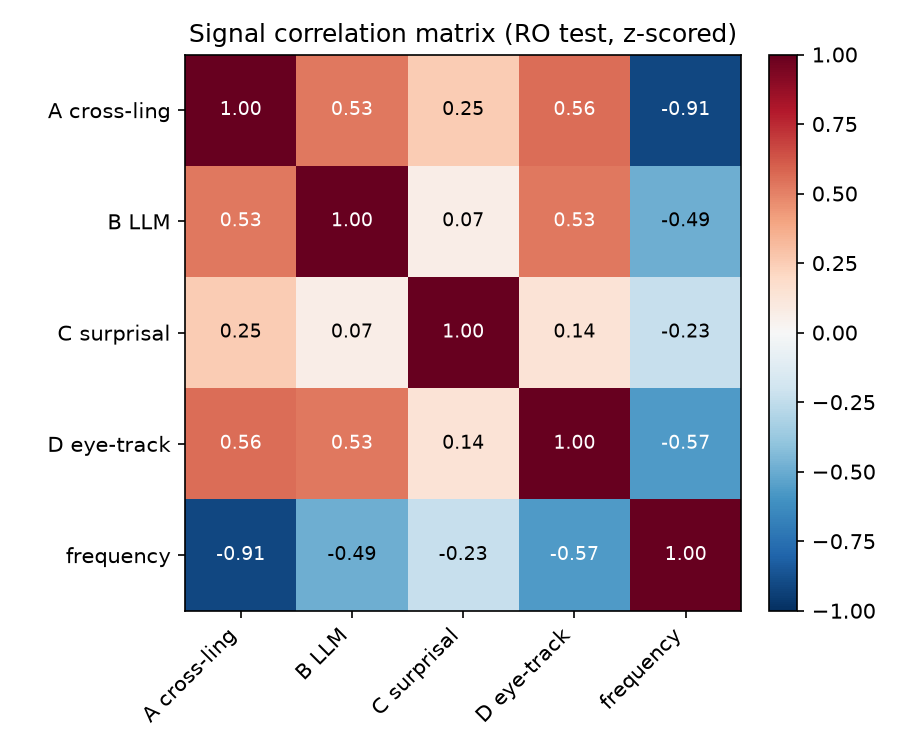
\includegraphics[width=\columnwidth]{fig_corr_matrix.png}
\caption{Correlation between the four signals and frequency on the Romanian test set. The rating (B) and surprisal
(C) are nearly independent; the cross-lingual signal (A) tracks frequency closely.}
\label{fig:corr}
\end{figure}

\begin{figure}[tbp]
\centering
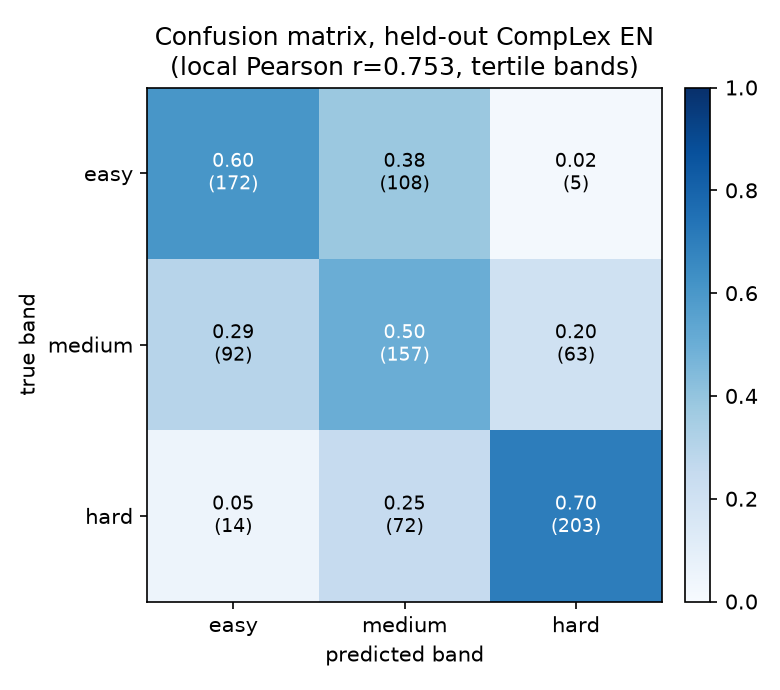
\includegraphics[width=0.8\columnwidth]{fig_confusion.png}
\caption{In-source check: on held-out English words, the regressor sorts complexity into easy/medium/hard bands
with a clearly diagonal confusion matrix.}
\label{fig:confusion}
\end{figure}

\begin{table}[tbp]
\centering\small
\begin{tabular}{lcc}
\toprule
\textbf{Configuration} & \textbf{Score} & \textbf{$\Delta$} \\
\midrule
Predict a constant (the mean) & 0.00 & --- \\
Surface features only (zero-shot RO) & 10.27 & +10.27 \\
\;+ eye-tracking (no imported res.) & 41.76 & +31.49 \\
\;+ cross-lingual A + LLM B & 64.52 & +22.76 \\
\;+ surprisal C & 64.81 & +0.29 \\
\;+ lemma-frequency fix (in A) & 68.90 & +4.09 \\
\;+ eye-tracking PCA D & \textbf{69.74} & +0.84$^{\dagger}$ \\
\bottomrule
\end{tabular}
\caption{Shared-task score (Equation~\ref{eq:metric}), built one component at a time; $\Delta$ is the marginal
contribution of each component. Predicting one constant gives no correlation, hence $0$. The first two rows use
only resources the shared task provides, so the imported signals account for $(69.74-41.76)/69.74 \approx 40\%$ of
the final score. $^{\dagger}$This delta is the maximum of the sweep that selected $w_D$ and should be read as an
upper bound (Section~\ref{sec:tuning}).}
\label{tab:ablation}
\end{table}

\begin{table}[tbp]
\centering\small
\begin{tabular}{lc}
\toprule
\textbf{Predictor on the 14 items} & \textbf{Pearson $r$} \\
\midrule
Zipf frequency, inflected form & $-0.606$ \\
Zipf frequency, lemma-corrected & $+0.092$ \\
\midrule
A cross-lingual, English source & $0.891$ \\
A cross-lingual, Romance source & $0.759$ \\
A ensemble & $0.838$ \\
B language-model rating & $0.615$ \\
\midrule
A+B, uniform weights (untuned) & $0.894$ \\
A+B, tuned weights & $\mathbf{0.913}$ \\
\bottomrule
\end{tabular}
\caption{Pearson $r$ against the gold labels of the 14 Romanian items, which took no part in weight selection.
Complexity falls as frequency rises, so a negative $r$ is the expected direction for the frequency rows and a
positive one for the model signals. Bootstrap $95\%$ CIs over $10{,}000$ resamples: $[0.661, 0.967]$ for the
untuned fusion and $[0.663, 0.975]$ for the tuned one; a permutation test over $20{,}000$ shuffles gives
$p < 0.0001$ for the latter. Signals C and D are absent: surprisal was not computed for these items and only $2$
of the $14$ have eye-tracking.}
\label{tab:ro14}
\end{table}

\begin{table}[tbp]
\centering\small
\begin{tabular}{lcc}
\toprule
\textbf{Signal} & \textbf{SHAP importance} & \textbf{weight} \\
\midrule
A cross-lingual & 0.061 & 44\% \\
B LLM rating & 0.034 & 29\% \\
D eye-tracking & 0.017 & 20\% \\
C surprisal & 0.006 & 6\% \\
\bottomrule
\end{tabular}
\caption{Per-signal SHAP importance and the weight each signal gets in the final average. The two orders agree;
SHAP describes the model, it does not choose the weights.}
\label{tab:signals}
\end{table}

\begin{table}[tbp]
\centering\small
\begin{tabular}{lc}
\toprule
\textbf{Eye-tracking metric} & \textbf{PC1 loading} \\
\midrule
Total fixation time (TFT) & 0.44 \\
Total fixation count (TFC) & 0.43 \\
First-pass reading time (FPRT) & 0.42 \\
First-pass fixation count (FPFC) & 0.39 \\
Re-reading time (RRT) & 0.35 \\
First-fixation duration (FFD) & 0.29 \\
Regression-path duration (RPD\_inc) & 0.28 \\
Incoming regressions (TRC\_in) & 0.13 \\
\bottomrule
\end{tabular}
\caption{Weight of each eye-tracking metric in the reading-effort score (loadings on PC1, which explains $62\%$ of
the variance). All loadings are positive: one ``more effort = more complex'' axis.}
\label{tab:pca}
\end{table}

\section{What Did Not Work}
\label{sec:negative}

Table~\ref{tab:fail} lists the attempts that failed, and two of them
carry a lesson beyond this system.

\paragraph{Fine-tuning is worse than freezing.}
Every form of fine-tuning we tried --- full fine-tuning and LoRA, over
a sweep of learning rates, epochs and ranks --- transferred worse than
the frozen encoder ($0.461$ and $0.462$ against $0.515$). With no
target-language labels, fine-tuning can only adapt to the source
language, and in doing so it degrades the cross-lingual alignment that
the transfer depends on. This is the behaviour \citet{peters-etal-2019-tune}
report when the target task is distant from the source, and it is worth
stating plainly because the default move in a cross-lingual pipeline is
to fine-tune \citep{pires-etal-2019-multilingual}.

\paragraph{In-source validation does not predict transfer to Romanian.}
Three configurations beat the frozen XLM-R baseline on in-source
transfer and then lost on Romanian: a different encoder (e5), mid-layer
embeddings, and a Lasso regressor. The in-source check measures
transfer between English and Romance --- related, well-resourced
languages --- and that is evidently not the same problem as transfer
into Romanian. In a setting with no target-language development set
this is the uncomfortable conclusion: the validation signal available
is not the validation signal needed.

\paragraph{Prompting and extra features.}
Chain-of-thought and few-shot prompting added noise rather than signal;
at the $8$B scale chain-of-thought is not yet reliably helpful
\citep{wei2022cot}. Rarity measures and a range of part-of-speech,
named-entity and WordNet features proved redundant with frequency,
which is consistent with the SHAP picture in
Figure~\ref{fig:beeswarm}.

\begin{table}[tbp]
\centering\small
\begin{tabular}{lcc}
\toprule
\textbf{Attempt} & \textbf{in-source} & \textbf{score} \\
\midrule
\multicolumn{3}{l}{\emph{Fine-tuning} ($r_{\mathrm{EN}\rightarrow\mathrm{RO}^{*}}$)} \\
Frozen XLM-R (this work) & 0.515 & --- \\
Full fine-tune (best of sweep) & 0.461 & --- \\
LoRA (best of sweep) & 0.462 & --- \\
\midrule
\multicolumn{3}{l}{\emph{Representation and regressor} ($\bar{r}_{\mathrm{transfer}}$)} \\
Frozen XLM-R (this work) & 0.551 & 69.74 \\
Encoder swap (e5) & 0.586 & 63.00 \\
Mid-layer embeddings & 0.556 & 64.49 \\
Lasso regressor & 0.569 & 64.28 \\
\midrule
\multicolumn{3}{l}{\emph{Prompting}} \\
LLM few-shot prompt & --- & 63.31 \\
\bottomrule
\end{tabular}
\caption{Failed attempts. The two blocks use different in-source measures and are not comparable across blocks:
$r_{\mathrm{EN}\rightarrow\mathrm{RO}^{*}}$ is the one-directional English-to-Romance transfer correlation, and
$\bar{r}_{\mathrm{transfer}}$ averages both directions. Within the second block, every variant that beats the
frozen baseline in-source loses on the shared-task score.}
\label{tab:fail}
\end{table}

\section{Conclusions}
\label{section:conclusions}

The absence of Romanian training data did not merely constrain the
design, it determined it: with no labels to fit and no development set
to select on, the only remaining move is to import complexity knowledge
from elsewhere and combine several independent imports. Four such
signals --- a frozen multilingual encoder, a language-model rating,
surprisal, and gaze --- reach $69.74$ on the shared-task metric and
$r = 0.913$ on the only Romanian labels available, without a single
target-language annotation.

Three findings generalise beyond Romanian. A lemma-frequency correction
is worth more than any other single component ($+4.09$) for a
morphologically rich language, subject to the scope condition of
Section~\ref{sec:14items}. Fine-tuning a multilingual encoder without
target labels is actively harmful, and freezing it is the stronger
default. And in-source validation, the only validation a zero-label
setting affords, does not reliably predict transfer to the target
language --- which is the finding we would most want future work in
this setting to take seriously.

\section*{Limitations}

\paragraph{Three weights were selected on the evaluation score.}
The setting provides no development set, so the three fusion weights
and the two calibration constants of Equation~\ref{eq:calib} were
chosen against the public leaderboard rather than held-out data. We
have bounded this in Section~\ref{sec:tuning} --- the calibration
cannot influence $r$, the response surface is flat, and the tuning is
worth $0.019$ of $r$ on labels it never saw --- but bounding is not
eliminating. The $69.74$ headline figure and, in particular, the
$+0.84$ credited to eye-tracking retain an unquantified optimistic
bias. A private-leaderboard evaluation would settle this and was not
available to us.

\paragraph{The reported metric cannot be decomposed.}
The shared-task metric of Equation~\ref{eq:metric} sums $|r|$ and
$\max(0,R^2)$, and the leaderboard returns only the sum. Because the
test labels are not released, we cannot report $r$ and $R^2$ separately
for any configuration evaluated on the full test set, and comparisons
against work that reports standard correlation measures are therefore
indirect. The separate figures we do give come from the 14 labelled
items only.

\paragraph{The independent evaluation rests on 14 items.}
Fourteen labelled words are the entirety of the Romanian supervision
that exists for this task. The bootstrap interval for our headline
correlation on them, $[0.663, 0.975]$, is correspondingly wide, and a
single item is enough to reverse the sign of the frequency baselines,
as Section~\ref{sec:14items} shows. Those items also cover only two of
the four signals --- surprisal was never computed for them and only two
carry eye-tracking --- so the fusion they validate is not the fusion we
submit. They were additionally consulted as a sanity check during
development, which makes them independent of the weight tuning but not
a pristine test set.

\paragraph{The eye-tracking analysis is partly circular.}
Because only $2$ of the $14$ labelled items have gaze data, the
early-versus-late analysis in Section~\ref{sec:results} could not be
validated against gold complexity. It uses the system's own predictions
as the complexity proxy over the $1509$ test words that have gaze, so
it establishes that late gaze measures carry information the other
signals lack \emph{relative to what our model predicts}, not relative
to human judgement. Gaze coverage is also not missing at random: the
$78$ words without fixations are shorter and more frequent than
average (mean Zipf $4.45$ against $4.20$; length $6.91$ against
$7.57$), because frequent short words are skipped, so the signal is
systematically absent exactly where it would matter least --- and its
absence is itself informative in a way the PCA score does not capture.

\paragraph{The lemma-frequency correction has a scope condition.}
Substituting lemma frequency assumes an inflected form inherits its
difficulty from its lemma. Section~\ref{sec:14items} documents a case
where this fails --- a simple-perfect verb form that is difficult
because of its inflection --- and we have not measured how often such
forms occur, since doing so would require Romanian labels. The
correction should be expected to help on average and to fail
systematically on archaic, literary or otherwise marked morphology.

\paragraph{The approach assumes resources that not every language has.}
The system needs an instruction-tuned language model in the target
language, a frequency list with lemma coverage, and annotated
complexity data in a related language. Romanian has all three, and the
shared task supplied the eye-tracking data, which is the least portable
of the four signals: gaze corpora exist for few languages, and
collecting them is expensive. A language lacking any of these would be
left with a proper subset of our signals, and we have not measured how
the fusion degrades under such a subset.

\paragraph{One target language, one domain.}
All results are for Romanian, on the texts of a single shared task.
The claims we expect to generalise --- that a frozen encoder beats
fine-tuning without target labels, and that in-source validation
misleads --- are supported here by one language pair each, and neither
has been tested on a second morphologically rich language.

\bibliography{custom}

\end{document}
